\documentclass[tikz, border=3pt]{standalone}
\usepackage{tikz}
\usetikzlibrary{decorations.pathreplacing,patterns, arrows, arrows.meta, shapes}
\definecolor{greengreen}{rgb}{0.0, 0.42, 0.24}
%%%%%%%%%%%%%%%%%%%%%%%%%%%%%%%%%%%%%%%%%%%%%%%%%%%%%%%%%%%%%%%%%
\begin{document}
%%%%%%%%%%%%%%%%%%%%%%%%%%%%%%%%%%%%%%%%%%%%%%%%%%%%%%%%%%%%%%%%%
\tikzset{>={Latex[width=3mm,length=3mm]}}
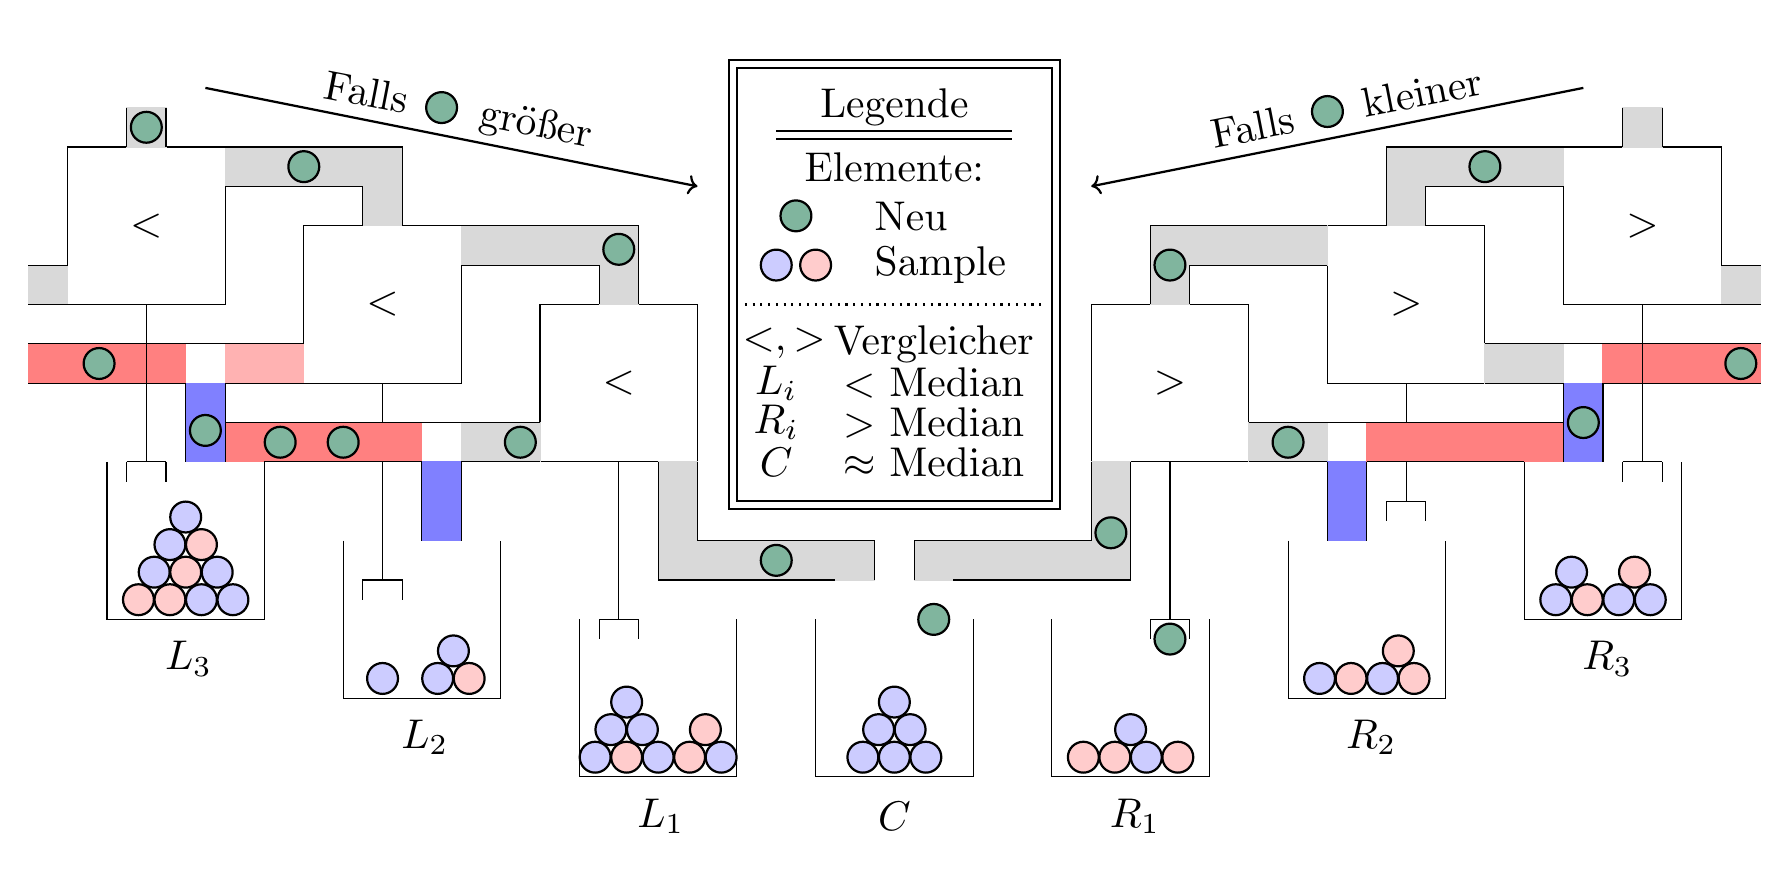
\begin{tikzpicture}[every node/.style={align=center, thick, scale=1.5},
red/.style={fill=red,draw,circle,inner sep=0pt},
blue/.style={fill=blue,draw,circle,inner sep=0pt},
 text width = .35cm]
%================================================================
% ==== Sets
% Median Candidates
\draw (-1, 3) -- (-1, 1) -- (1, 1) -- (1, 3);

% Subsets L_i
\foreach \x/\y in {3.5/5, 6.5/6, 9.5/7}
  \draw (-1 -\x, 0 +\y) -- (1 - \x, 0 + \y) -- (1 - \x, 1.5 + \y);

\foreach \x/\y in {3.5/5, 6.5/6, 9.5/7}
  \draw (1 -\x, 2 +\y) -- (0.25 - \x, 2 + \y);

\foreach \x/\y in {3.5/5, 6.5/6, 9.5/7}
  \draw (-0.25 -\x, 2 +\y) -- (-1 - \x, 2 + \y) -- (-1 - \x, 0.5 + \y);

% Subsets R_i

\foreach \x/\y in {3.5/5, 6.5/6, 9.5/7}
  \draw (1 +\x, 0.5 +\y) -- (1 + \x, 2 + \y) -- (0.25 + \x, 2 + \y);

\foreach \x/\y in {3.5/5, 6.5/6, 9.5/7}
  \draw (-0.25 +\x, 2 +\y) -- (-1 + \x, 2 + \y) -- (-1 + \x, 0 + \y) -- (1 + \x, 0 + \y);

% Arm
\draw (-6.5, 6) -- (-6.5, 3.5);
\draw (-6.25, 3.25) -- (-6.25, 3.5) -- (-6.75, 3.5) -- (-6.75, 3.25);


%================================================================
% Operators L_i
\foreach \x/\y in {3/1, 6/2, 9/3}
  \draw (-1 -\x, 2 +\y) -- (-1 - \x, 0 + \y) -- (1 - \x, 0 + \y) -- (1 - \x, 2 + \y);

\draw[pattern=north east lines, color=gray!30] (-10.5, 7) rectangle (-11, 7.5);
\draw (-10.5, 7) -- (-11, 7);
\draw (-10.5, 7.5) -- (-11, 7.5);

\draw[pattern=north east lines, color=red!30] (-7.5, 6) rectangle (-8.5, 6.5);
\draw[pattern=north east lines, color=blue!50] (-8.5, 6) rectangle (-9, 5);
\draw[pattern=north east lines, color=red!50] (-9, 6) rectangle (-11, 6.5);

\draw[pattern=north east lines, color=gray!30] (-4.5, 5) rectangle (-5.5, 5.5);
\draw[pattern=north east lines, color=blue!50] (-5.5, 5) rectangle (-6, 4);
\draw[pattern=north east lines, color=red!50] (-6, 5) rectangle (-8.5, 5.5);


\draw[pattern=north east lines, color=gray!30] (-9.75, 9) rectangle (-9.25, 9.5);
\draw (-9.75, 9) -- (-9.75, 9.5);
\draw (-9.25, 9) -- (-9.25, 9.5);


\draw[pattern=north east lines, color=gray!30] (-8.5, 9) rectangle (-6.25, 8.5);
\draw[pattern=north east lines, color=gray!30] (-6.75, 8.5) rectangle (-6.25, 8);
\draw (-8.5, 9) -- (-6.25, 9) -- (-6.25, 8);
\draw (-8.5, 8.5) -- (-6.75, 8.5) -- (-6.75, 8);

\draw[pattern=north east lines, color=gray!30] (-5.5, 8) rectangle (-3.25, 7.5);
\draw[pattern=north east lines, color=gray!30] (-3.75, 7.5) rectangle (-3.25, 7);
\draw (-5.5, 8) -- (-3.25, 8) -- (-3.25, 7);
\draw (-5.5, 7.5) -- (-3.75, 7.5) -- (-3.75, 7);

\draw[pattern=north east lines, color=gray!30] (-2.5, 5) rectangle (-3, 3.5);
\draw[pattern=north east lines, color=gray!30] (-2.5, 4) rectangle (-0.25, 3.5);
\draw (-3, 5) -- (-3, 3.5) -- (-0.75, 3.5);
\draw (-2.5, 5) -- (-2.5, 4) -- (-0.25, 4) -- (-0.25, 3.5);

% Tubes
\draw (-2.5, 7) -- (-2.5, 6.5);
\draw (-4.5, 5) -- (-5.5, 5);
\draw (-6, 5) -- (-8, 5);
\draw (-4.5, 5.5) -- (-8.5, 5.5) -- (-8.5, 5);
\draw (-7.5, 6) -- (-8.5, 6);
\draw (-9, 6) -- (-11, 6);
\draw (-7.5, 6.5) -- (-11, 6.5);
\draw (-8.5, 5.5) -- (-8.5, 6);
\draw (-9, 5) -- (-9, 6);
\draw (-5.5, 5) -- (-5.5, 4);
\draw (-6, 5) -- (-6, 4);


\foreach \x/\y in {3.5/5, 9.5/7}
  \draw (-\x, \y) -- (-\x, \y - 2);

\foreach \x/\y in {3.5/5, 9.5/7}
  \draw (-\x - 0.25, \y - 2) -- (-\x + 0.25, \y - 2);

\foreach \x/\y in {3.5/5, 9.5/7}
  \draw (-\x - 0.25, \y - 2) -- (-\x - 0.25, \y - 2.25);

\foreach \x/\y in {3.5/5, 9.5/7}
  \draw (-\x + 0.25, \y - 2) -- (-\x + 0.25, \y - 2.25);

\draw (6.5, 6) -- (6.5, 4.5);
\draw (6.25, 4.25) -- (6.25, 4.5) -- (6.75, 4.5) -- (6.75, 4.25);

%================================================================
  \foreach \x/\y in {3/1, 6/2, 9/3}
    \draw (-1 +\x, 2 +\y) -- (-1 + \x, 0 + \y) -- (1 + \x, 0 + \y) -- (1 + \x, 2 + \y);

\draw[pattern=north east lines, color=gray!30] (10.5, 7) rectangle (11, 7.5);
\draw (10.5, 7) -- (11, 7);
\draw (10.5, 7.5) -- (11, 7.5);

\draw[pattern=north east lines, color=gray!30] (7.5, 6) rectangle (8.5, 6.5);
\draw[pattern=north east lines, color=blue!50] (8.5, 6) rectangle (9, 5);
\draw[pattern=north east lines, color=red!50] (9, 6) rectangle (11, 6.5);

\draw[pattern=north east lines, color=gray!30] (4.5, 5) rectangle (5.5, 5.5);
\draw[pattern=north east lines, color=blue!50] (5.5, 5) rectangle (6, 4);
\draw[pattern=north east lines, color=red!50] (6, 5) rectangle (8.5, 5.5);

\draw[pattern=north east lines, color=gray!30] (9.75, 9) rectangle (9.25, 9.5);
\draw (9.75, 9) -- (9.75, 9.5);
\draw (9.25, 9) -- (9.25, 9.5);

\draw[pattern=north east lines, color=gray!30] (8.5, 9) rectangle (6.25, 8.5);
\draw[pattern=north east lines, color=gray!30] (6.75, 8.5) rectangle (6.25, 8);
\draw (8.5, 9) -- (6.25, 9) -- (6.25, 8);
\draw (8.5, 8.5) -- (6.75, 8.5) -- (6.75, 8);

\draw[pattern=north east lines, color=gray!30] (5.5, 8) rectangle (3.25, 7.5);
\draw[pattern=north east lines, color=gray!30] (3.75, 7.5) rectangle (3.25, 7);
\draw (5.5, 8) -- (3.25, 8) -- (3.25, 7);
\draw (5.5, 7.5) -- (3.75, 7.5) -- (3.75, 7);

\draw[pattern=north east lines, color=gray!30] (2.5, 5) rectangle (3, 3.5);
\draw[pattern=north east lines, color=gray!30] (2.5, 4) rectangle (0.25, 3.5);
\draw (3, 5) -- (3, 3.5) -- (0.75, 3.5);
\draw (2.5, 5) -- (2.5, 4) -- (0.25, 4) -- (0.25, 3.5);

\draw (2.5, 7) -- (2.5, 6.5);
\draw (4.5, 5) -- (5.5, 5);
\draw (6, 5) -- (8, 5);
\draw (4.5, 5.5) -- (8.5, 5.5) -- (8.5, 5);
\draw (7.5, 6) -- (8.5, 6);
\draw (9, 6) -- (11, 6);
\draw (7.5, 6.5) -- (11, 6.5);
\draw (8.5, 5.5) -- (8.5, 6);
\draw (9, 5) -- (9, 6);
\draw (5.5, 5) -- (5.5, 4);
\draw (6, 5) -- (6, 4);

% Arm
\foreach \x/\y in {3.5/5, 9.5/7}
  \draw (\x, \y) -- (\x, \y - 2);

\foreach \x/\y in {3.5/5, 9.5/7}
  \draw (\x - 0.25, \y - 2) -- (\x + 0.25, \y - 2);

\foreach \x/\y in {3.5/5, 9.5/7}
  \draw (\x - 0.25, \y - 2) -- (\x - 0.25, \y - 2.25);

\foreach \x/\y in {3.5/5, 9.5/7}
  \draw (\x + 0.25, \y - 2) -- (\x + 0.25, \y - 2.25);


%================================================================

% ==== Legend
\draw[thick] (-2, 4.5) rectangle (2, 10);
\draw[thick] (-2.1, 4.4) rectangle (2.1, 10.1);

\node[very thick, text width=3cm] at (0, 9.5) {Legende};
\draw[-, thick] (-1.5, 9.1) -- (1.5, 9.1);
\draw[-, thick] (-1.5, 9.2) -- (1.5, 9.2);

\node[thick, text width=3cm] at (0, 8.75) {Elemente:};

\node[circle,fill=greengreen!50,draw, inner sep=0pt, scale = 0.75] at (-1.25, 8.125) {};
\node[thick, text width=3cm, align=left] at (2, 8.125) {Neu};

\node[circle,fill=blue!20,draw, inner sep=0pt, scale = 0.75] at (-1.5, 7.5) {};
\node[circle,fill=red!20,draw, inner sep=0pt, scale = 0.75] at (-1, 7.5) {};
\node[thick, text width=3cm, align=left] at (2, 7.5) {Sample};

\draw[thick, dotted] (-1.9, 7) -- (1.9, 7);

\node[thick, text width=3cm] at (-1.4, 6.5) {$<, >$};
\node[thick, text width=3cm] at (0.5, 6.5) {Vergleicher};

\node[thick, text width=3cm] at (-1.5, 6) {$L_i$};
\node[thick, text width=3cm] at (0.5, 6) {$<$ Median};

\node[thick, text width=3cm] at (-1.5, 5.5) {$R_i$};
\node[thick, text width=3cm] at (0.5, 5.5) {$>$ Median};

\node[thick, text width=3cm] at (-1.5, 5) {$C$};
\node[thick, text width=4cm] at (0.5, 5) {$\approx$ Median};



%================================================================

% C
\node[circle,fill=blue!20,draw, inner sep=0pt, scale = 0.75] at (0, 1.25) {};
\node[circle,fill=blue!20,draw, inner sep=0pt, scale = 0.75] at (0.4, 1.25) {};
\node[circle,fill=blue!20,draw, inner sep=0pt, scale = 0.75] at (-0.4, 1.25) {};
\node[circle,fill=blue!20,draw, inner sep=0pt, scale = 0.75] at (0.2, 1.6) {};
\node[circle,fill=blue!20,draw, inner sep=0pt, scale = 0.75] at (-0.2, 1.6) {};
\node[circle,fill=blue!20,draw, inner sep=0pt, scale = 0.75] at (0, 1.95) {};
\node[circle,fill=greengreen!50,draw, inner sep=0pt, scale = 0.75] at (0.5, 3) {};
\node[circle,fill=greengreen!50,draw, inner sep=0pt, scale = 0.75] at (-1.5, 3.75) {};


% R_1
\node[circle,fill=red!20,draw, inner sep=0pt, scale = 0.75] at (3.6, 1.25) {};
\node[circle,fill=red!20,draw, inner sep=0pt, scale = 0.75] at (2.4, 1.25) {};
\node[circle,fill=greengreen!50,draw, inner sep=0pt, scale = 0.75] at (3.5, 2.75) {};
\node[circle,fill=blue!20,draw, inner sep=0pt, scale = 0.75] at (3.2, 1.25) {};
\node[circle,fill=red!20,draw, inner sep=0pt, scale = 0.75] at (2.8, 1.25) {};
\node[circle,fill=blue!20,draw, inner sep=0pt, scale = 0.75] at (3, 1.6) {};

\node[circle,fill=greengreen!50,draw, inner sep=0pt, scale = 0.75] at (3.5, 7.5) {};

\node[circle,fill=greengreen!50,draw, inner sep=0pt, scale = 0.75] at (5, 5.25) {};

\node[circle,fill=blue!20,draw, inner sep=0pt, scale = 0.75] at (5.4, 2.25) {};
\node[circle,fill=red!20,draw, inner sep=0pt, scale = 0.75] at (5.8, 2.25) {};
\node[circle,fill=blue!20,draw, inner sep=0pt, scale = 0.75] at (6.2, 2.25) {};
\node[circle,fill=red!20,draw, inner sep=0pt, scale = 0.75] at (6.6, 2.25) {};
\node[circle,fill=red!20,draw, inner sep=0pt, scale = 0.75] at (6.4, 2.6) {};

% R_i right
\node[circle,fill=blue!20,draw, inner sep=0pt, scale = 0.75] at (8.4, 3.25) {};
\node[circle,fill=red!20,draw, inner sep=0pt, scale = 0.75] at (8.8, 3.25) {};
\node[circle,fill=blue!20,draw, inner sep=0pt, scale = 0.75] at (8.6, 3.6) {};
\node[circle,fill=blue!20,draw, inner sep=0pt, scale = 0.75] at (9.2, 3.25) {};
\node[circle,fill=blue!20,draw, inner sep=0pt, scale = 0.75] at (9.6, 3.25) {};
\node[circle,fill=red!20,draw, inner sep=0pt, scale = 0.75] at (9.4, 3.6) {};


\node[circle,fill=greengreen!50,draw, inner sep=0pt, scale = 0.75] at (8.75, 5.5) {};
\node[circle,fill=greengreen!50,draw, inner sep=0pt, scale = 0.75] at (10.75, 6.25) {};

\node[circle,fill=greengreen!50,draw, inner sep=0pt, scale = 0.75] at (7.5, 8.75) {};



% Left

\node[circle,fill=blue!20,draw, inner sep=0pt, scale = 0.75] at (-3.8, 1.25) {};
\node[circle,fill=red!20,draw, inner sep=0pt, scale = 0.75] at (-3.4, 1.25) {};
\node[circle,fill=blue!20,draw, inner sep=0pt, scale = 0.75] at (-3, 1.25) {};
\node[circle,fill=red!20,draw, inner sep=0pt, scale = 0.75] at (-2.6, 1.25) {};
\node[circle,fill=blue!20,draw, inner sep=0pt, scale = 0.75] at (-2.2, 1.25) {};

\node[circle,fill=blue!20,draw, inner sep=0pt, scale = 0.75] at (-3.6, 1.6) {};
\node[circle,fill=blue!20,draw, inner sep=0pt, scale = 0.75] at (-3.2, 1.6) {};
\node[circle,fill=red!20,draw, inner sep=0pt, scale = 0.75] at (-2.4, 1.6) {};
\node[circle,fill=blue!20,draw, inner sep=0pt, scale = 0.75] at (-3.4, 1.95) {};


\node[circle,fill=greengreen!50,draw, inner sep=0pt, scale = 0.75] at (-3.5, 7.7) {};
\node[circle,fill=greengreen!50,draw, inner sep=0pt, scale = 0.75] at (2.75, 4.1) {};

\node[circle,fill=greengreen!50,draw, inner sep=0pt, scale = 0.75] at (-4.75, 5.25) {};
\node[circle,fill=greengreen!50,draw, inner sep=0pt, scale = 0.75] at (-7, 5.25) {};
\node[circle,fill=greengreen!50,draw, inner sep=0pt, scale = 0.75] at (-7.8, 5.25) {};


\node[circle,fill=blue!20,draw, inner sep=0pt, scale = 0.75] at (-6.5, 2.25) {};
\node[circle,fill=blue!20,draw, inner sep=0pt, scale = 0.75] at (-5.8, 2.25) {};
\node[circle,fill=red!20,draw, inner sep=0pt, scale = 0.75] at (-5.4, 2.25) {};
\node[circle,fill=blue!20,draw, inner sep=0pt, scale = 0.75] at (-5.6, 2.6) {};



\node[circle,fill=greengreen!50,draw, inner sep=0pt, scale = 0.75] at (-7.5, 8.75) {};
\node[circle,fill=greengreen!50,draw, inner sep=0pt, scale = 0.75] at (-8.75, 5.4) {};


\node[circle,fill=red!20,draw, inner sep=0pt, scale = 0.75] at (-9.6, 3.25) {};
\node[circle,fill=red!20,draw, inner sep=0pt, scale = 0.75] at (-9.2, 3.25) {};
\node[circle,fill=blue!20,draw, inner sep=0pt, scale = 0.75] at (-8.8, 3.25) {};
\node[circle,fill=blue!20,draw, inner sep=0pt, scale = 0.75] at (-8.4, 3.25) {};
\node[circle,fill=blue!20,draw, inner sep=0pt, scale = 0.75] at (-9.4, 3.6) {};
\node[circle,fill=red!20,draw, inner sep=0pt, scale = 0.75] at (-9, 3.6) {};
\node[circle,fill=blue!20,draw, inner sep=0pt, scale = 0.75] at (-8.6, 3.6) {};
\node[circle,fill=blue!20,draw, inner sep=0pt, scale = 0.75] at (-9.2, 3.95) {};
\node[circle,fill=red!20,draw, inner sep=0pt, scale = 0.75] at (-8.8, 3.95) {};
\node[circle,fill=blue!20,draw, inner sep=0pt, scale = 0.75] at (-9, 4.3) {};


\node[circle,fill=greengreen!50,draw, inner sep=0pt, scale = 0.75] at (-9.5, 9.25) {};
\node[circle,fill=greengreen!50,draw, inner sep=0pt, scale = 0.75] at (-10.1, 6.25) {};

\node at (0, 0.5) {$C$};

\node at (-3, 0.5) {$L_1$};
\node at (-6, 1.5) {$L_2$};
\node at (-9, 2.5) {$L_3$};
\node at (3, 0.5) {$R_1$};
\node at (6, 1.5) {$R_2$};
\node at (9, 2.5) {$R_3$};

\node at (-3.5, 6) {$<$};
\node at (-6.5, 7) {$<$};
\node at (-9.5, 8) {$<$};
\node at (3.5, 6) {$>$};
\node at (6.5, 7) {$>$};
\node at (9.5, 8) {$>$};

\draw[thick, ->] (-8.75, 9.75) -- (-2.5, 8.5);
\node[thick, text width=3cm, rotate=349] at (-6.7, 9.7) {Falls};
\node[circle,fill=greengreen!50,draw, inner sep=0pt, scale = 0.75] at (-5.75, 9.5) {};
\node[thick, text width=3cm, rotate=349] at (-4.55, 9.26) {größer};

\draw[thick, ->]  (8.75, 9.75) -- (2.5, 8.5);
\node[thick, text width=3cm, rotate=11] at (6.7, 9.7) {kleiner};
\node[circle,fill=greengreen!50,draw, inner sep=0pt, scale = 0.75] at (5.5, 9.45) {};
\node[thick, text width=3cm, rotate=11] at (4.55, 9.26) {Falls};



% Arrows: Green / Left
%\foreach \x/\y in {-3/6.95, -6/7.95, -9/8.95}
%  \draw[color=greengreen, ->, thick] (\x - 0.5, \y) -- (\x - 0.5, \y - 0.5);
%\foreach \x/\y in {-3/5.05, -6/6.05, -9/7.05}
%  \draw[color=greengreen, ->, thick] (\x - 0.5, \y) -- (\x - 0.5, \y + 0.5);
%\foreach \x/\y in {-5.5/7.75, -8.5/8.75}
%  \draw[color=greengreen, ->, thick] (\x - 0.55, \y) -- (\x - 0.05, \y);
%\foreach \x/\y in {-3.95/5.25, -6.95/6.25, -9.95/7.25}
%  \draw[color=greengreen, ->, thick] (\x, \y) -- (\x - 0.5, \y);
%\draw[color=greengreen, ->, thick] (-2.75, 5.50) -- (-2.75, 5.05);

% Arrows: Green / Right
%\foreach \x/\y in {3/6.95, 6/7.95, 9/8.95}
%  \draw[color=greengreen, ->, thick] (\x + 0.5, \y) -- (\x + 0.5, \y - 0.5);
%foreach \x/\y in {3/5.05, 6/6.05, 9/7.05}
%  \draw[color=greengreen, ->, thick] (\x + 0.5, \y) -- (\x + 0.5, \y + 0.5);
%\foreach \x/\y in {5.5/7.75, 8.5/8.75}
%  \draw[color=greengreen, ->, thick] (\x + 0.55, \y) -- (\x + 0.05, \y);
%\foreach \x/\y in {3.95/5.25, 6.95/6.25, 9.95/7.25}
%  \draw[color=greengreen, ->, thick] (\x, \y) -- (\x + 0.5, \y);
%\draw[color=greengreen, ->, thick] (2.75, 5.50) -- (2.75, 5.05);

%================================================================
\end{tikzpicture}
%%%%%%%%%%%%%%%%%%%%%%%%%%%%%%%%%%%%%%%%%%%%%%%%%%%%%%%%%%%%%%%%%
\end{document}
%%%%%%%%%%%%%%%%%%%%%%%%%%%%%%%%%%%%%%%%%%%%%%%%%%%%%%%%%%%%%%%%%
